  %!TEX root = ../main.tex


\subsection{Univariate modeling of factor returns} % (fold)
\label{subsec:univariate_modeling}

We proceed by estimating models of each factor's return series and attempt to capture the effects of non-normality, autocorrelation and volatility clustering that were established in \autoref{sec:data}. By estimating ARMA-GARCH, we can characterize and filter these effects. Furthermore, we can incorporate the effects in conditional forecasts. In this section, we describe the general structure of our models, our systematic model selection approach and the estimation results.

\subsubsection{General univariate model: ARMA-GJR-GARCH} % (fold)
\label{subsubsec:general_univariate_model_gjr_garch}

The ARMA-GARCH is a broad model family designed to eliminate predictable components of financial return series. The models use autoregressive and moving average lags to capture serial correlation in return data (ARMA), as well as autoregressive and moving average lags to capture ARCH effects in residuals from the mean equation (GARCH). ARCH effects are also referred to as volatility clustering, due to the persistence in magnitude of return shocks. Shocks in financial return series are often not homoskedastic, and the heteroskedasticy tends to exhibit serial correlation. We evaluate the GJR-GARCH model of~\textcite{glosten1993relation}, which is a parsimonious extension of the standard GARCH(1, 1) model of~\autocite{Bollerslev1986}. The GJR-GARCH is designed to also capture leverage effects~\autocite{glosten1993relation}, i.e. when positive and negative return shocks have different impact on future volatility~\autocite{Black1976}.

We estimate conditional mean equations \emph{up to} ARMA(3, 3):
\begin{align}
  r_t &=
    \mu +
    \sum^p \phi_p r_{t - p} +
    \sum^q \theta_q \epsilon_{t - q} + 
    \epsilon_t
\end{align}
where $r_t$ are log returns. The conditional volatility evolves according to the GJR-GARCH specification:
\begin{align}
  \epsilon_t &= \sigma_t z_t \\
  \sigma_t^2 &=
    \omega +
    (\alpha + \eta I_{\epsilon_{t-1} \leq 0}) \epsilon_{t - 1}^2 +
    \beta \sigma^2_{t - 1}
\end{align}
where $I$ is an indicator function that is equal to one when $\epsilon_{t-1} \leq 0$. A positive $\eta$ captures the leverage effect by increasing the current period's volatility if the previous period's residual $\epsilon$ was below zero. A significant $\eta$ thus introduces asymmetric volatility in the model. For the market factor, it is expected that $\eta$ is positive, reflecting the leverage effect in the market itself and no impact from the short risk-free component. However, for the other factors, which are constructed as all-equity zero-cost long-short portfolios, the direction of $\eta$ is less obvious~\autocite{ChristoffersenLanglois2013}. If there are leverage effects for stocks in general, negative shocks will lead to more volatility than positive shocks in a portfolio of stocks. But in a zero-cost portfolio, the leverage effects of the long positions in stocks could be eliminated by the short positions in other firms. The level of the leverage effect in a zero-cost portfolio therefore depends on the relative strength of leverage effects in the long and short components.

The ARMA-GARCH models are estimated on each series using maximum likelihood estimation, taking an assumed conditional distribution of standardized returns $\{z_t\}$ as given. We evaluate models where the standardized residuals series $\{z_t\}$ are assumed to follow one of the following distributions: Standard normal, Student's \textit{t} with $\nu$ degrees of freedom and skewed Student's \textit{t} with $\nu$ degrees of freedom and skewness $\gamma$. The Student's t distribution allows for greater kurtosis (fatter tails) than the standard normal distribution, while skewed Student's \textit{t} also allows for additional asymmetry in the model's behavior beyond that introduced by the leverage effect. In the estimation, we also use variance targeting as proposed by~\textcite{EngleMezrich1995}, which is shown makes optimization faster and sometimes more certain to reach the global maximum. This means that $\omega$ is not estimated in the maximum likelihood setting, but instead set to 1 minus the persistence of the process times the sample mean of squared residuals, where the persistence is $\alpha + \beta$ for the GARCH.\footnote{Note that in the case of the GJR-GARCH for the Mkt-RF factor, the persistence is $\alpha + \beta + \eta \kappa$ where $\kappa$ is the probability that standardized residuals $z_t$ are below zero.}

% subsection general_univariate_model_gjr_garch (end)

\subsubsection{Factor specific model selection process} % (fold)
\label{subsubsec:selection_process}

Our selection process is as follows: For each factor strategy, we estimate GJR-GARCH models on the full dataset ($T = 2766$) up to ARMA(3, 3) and GARCH(1, 1) under normal, Student's t and skewed Student's t residuals, with and without $\eta$ fixed to zero (in which case we obtain the basic GARCH(1, 1) model). We then compute the Bayesian Information Criterion (BIC~\autocite{Schwarz1978}) for each factor strategy and specification and select the ARMA order with the lowest BIC as our primary candidates.

First, the candidate models are checked for remaining serial correlation and ARCH effects. Second, we examine whether there are significant leverage effects that warrant the use of a GJR-GARCH instead of a standard GARCH. Third, we use QQ-plots to control for misspecification in the residual process, and to find a suitable distribution for the standardized residuals $z_t$.

In a well-specified model, we expect there to be no significant serial correlation, ARCH effects or sign bias in the residuals. We employ weighted Ljung-Box, ARCH LM and sign bias tests that are detailed in \autoref{app:univariate_diagnostics}. Furthermore, the QQ-plots of the standardized residuals should show that their empirical distribution is comparable to the assumed theoretical distribution (be distributed around the 45 degree line).

% subsection selection_process (end)

  

\subsubsection{Model selection and estimation results}
\label{subsubsec:uni_selection_estimation_results}

The result of our selection and estimation procedure are presented in~\autoref{tab:garch_value} and~\autoref{tab:garch_nonvalue}. The Mkt-RF factor is the only model that requires a GJR-GARCH $\eta \neq 0$, while the remaining models are all standard GARCH (1, 1). The minimization of BIC leads to ARMA(0, 0) for Mkt-RF, ARMA(1, 0) for Mom and CMA and ARMA(1, 1) for the remaining factors HML, SMB, RMW. 

Based on these ARMA-GARCH specifications, the Ljung-Box and LM tests indicate no remaining serial correlation or ARCH effects, as all p-values are greater than our 5\% cut-off point. However, some p-values are quite close to the limit, including the Mkt-RF factor's Ljung-Box tests and the longer Ljung-Box tests of RMW and CMA. We also note that the Mkt-RF model selects order ARMA(0, 0), suggesting that it is hard to predict the 1-week-ahead return on the Mkt-RF based on serial correlation alone.

The lack of significant sign bias in the GARCH specifications for all models except Mkt-RF is interesting, but in line with the argument that any leverage effects could cancel out in a zero-cost long-short equity portfolio; the Mkt-RF is the only factor that is net-long equities and also exhibited the expected negative sign bias as a GARCH model. In \autoref{tab:garch_nonvalue}, we note that the sign bias of Mkt-RF has been eliminated in the GJR-GARCH model. 

The candidate specifications under normal and Student's \textit{t} distributed innovations all display misaligned QQ-plots, see \autoref{fig:qq_norm_std}. The empirical distributions deviate from the 45 degree theoretical lines, especially in the more extreme quantiles. This indicates asymmetry in the residual series. In unreported results, we have controlled that the misspecification of normal and Student's \textit{t} residuals is persistent even if GJR-GARCH models are fitted for all factors -- leverage effects can't explain the misspecification. By comparision (see~\autoref{fig:qq_ghst}), the QQ-plot with skewed Student's \textit{t} innovations seems to fit the data well. We proceed with skewed Student's \textit{t} residual distributions.

Now, we turn to the estimation results of the chosen ARMA-GJR-GARCH models in~\autoref{tab:garch_value} and~\autoref{tab:garch_nonvalue}. 

% TABLES NEED TO BE MODIFIED IN THE FOLLOWING WAYS
% 1) Change {tabular} to {tabularx}{\textwidth} and make leftmost column an X column
%     and change top and bottom \hline to \toprule \bottomrule
%
% paste the following at start but before & \multicolumn
%
% \begin{tabularx}{\textwidth}{@{\extracolsep{5pt}} X D{.}{.}{-3} D{.}{.}{-3} D{.}{.}{-3} } 
% \\[-1.8ex] \midrule
% \\[-1.8ex] 
%
% paste the following at end after R2 row but before Note row
% \bottomrule \\[-1.8ex] 
%
% 2) Change the variable names to greeks
% 3) Change specification names if needed
% 4) Change R2 to LLH and add similar lines for Ljung-Box and ARCH-LM
% 5) Add label and caption
% 6) Paste this to get table heading description
%
% \begin{tabularx}{\textwidth}{X}
% \\[-1.8ex]\toprule
%\\[-1.8ex] 
% text goes here
% \end{tabularx}
%
% 6) Copy the whole table, only change caption, label, factor/spec labels and (1)-(3) to (4)-(6)
%% TABLE 1 value factors HML, RMW, CMA
\begin{table}[!htbpp] \centering 
  \caption{ARMA-GARCH results: Mkt-RF, SMB, Mom} 
  \label{tab:garch_nonvalue} 
\begin{tabularx}{\textwidth}{X}
\\[-1.8ex]\toprule
\\[-1.8ex] 
\footnotesize Parameter estimates from ARMA-GARCH models on weekly returns 1963-2016. Heteroskedasticity robust standard errors in parentheses, following \textcite{White1982}. Mean equation: $r_t = \mu + \sum^p \phi_p r_{t-p} + \sum^q \theta_q \epsilon_{t-q} + \epsilon_{t}$ and variance equation: $\epsilon_t = \sigma_t z_t$ and $\sigma_t^2 = \omega + (\alpha + \eta I_{\epsilon_{t-1} \leq 0}) \epsilon_{t - 1}^2 + \beta \sigma^2_{t - 1}$. $\gamma$ and $\nu$ are the skewness and degree of freedom parameters of the skewed Student's \textit{t} innovations. $\eta$ is fixed at zero for SMB and Mom, as the sign bias test showed no significant misspecification of the GARCH. $\omega$ is set using variance targeting, following \textcite{EngleMezrich1995}. Ljung-Box and ARCH-LM tests are the weighted portmanteau tests from \textcite{FisherGallagher2012} and the sign bias test is from \textcite{EngleNg1993}.
\end{tabularx}
\begin{tabularx}{\textwidth}{@{\extracolsep{5pt}} X D{.}{.}{-3} D{.}{.}{-3} D{.}{.}{-3} } 
\\[-1.8ex]\midrule
\\[-1.8ex] 
 & \multicolumn{3}{c}{Factor series} \\ 
\cline{2-4} 
\\[-1.8ex] & \multicolumn{1}{c}{(1)} & \multicolumn{1}{c}{(2)} & \multicolumn{1}{c}{(3)}\\ 
\\[-1.8ex] & \multicolumn{1}{c}{Mkt-RF} & \multicolumn{1}{c}{SMB} & \multicolumn{1}{c}{Mom}\\ 
\hline \\[-1.8ex] 
 $\mu\,\,(percent)$ & 0.096^{***} & 0.026 & 0.128^{***} \\ 
  & (0.032) & (0.033) & (0.032) \\ 
  & & & \\ 
 $\phi_1$ &  & 0.772^{***} & 0.129^{***} \\ 
  &  & (0.046) & (0.027) \\ 
  & & & \\ 
 $\theta_1$ &  & -0.652^{***} &  \\ 
  &  & (0.056) & \\ 
  & & & \\ 
 $\alpha$ & 0.037^{**} & 0.115^{***} & 0.186^{***} \\ 
  & (0.015) & (0.023) & (0.003) \\ 
  & & & \\ 
 $\beta$ & 0.844^{***} & 0.841^{***} & 0.793^{***} \\ 
  & (0.006) & (0.035) & (0.004) \\ 
  & & & \\ 
 $\eta$ & 0.181^{***} & 0.000 & 0.000 \\ 
  & (0.023) &  &  \\ 
  & & & \\ 
 $\gamma$ & -2.482^{**} & -0.864 & -2.547 \\ 
  & (1.020) & (1.755) & (4.985) \\ 
  & & & \\ 
 $\nu$ & 12.170^{***} & 11.801 & 13.822 \\ 
  & (3.072) & (15.791) & (17.436) \\ 
  & & & \\ 
 $\omega\,\,(per\,mil)$ & 0.016 & 0.006 & 0.007 \\ 
\hline \\[-1.8ex] 
Observations & \multicolumn{1}{c}{2,766} & \multicolumn{1}{c}{2,766} & \multicolumn{1}{c}{2,766} \\ 
LLH & \multicolumn{1}{c}{7,051} & \multicolumn{1}{c}{8,568} & \multicolumn{1}{c}{7,941} \\ 
Unconditional volatility & \multicolumn{1}{c}{0.022} & \multicolumn{1}{c}{0.010} & \multicolumn{1}{c}{0.017} \\
Variance persistence & \multicolumn{1}{c}{0.966} & \multicolumn{1}{c}{0.957} & \multicolumn{1}{c}{0.979} \\
Ljung-Box [5] p-value & \multicolumn{1}{c}{0.108} & \multicolumn{1}{c}{0.307} & \multicolumn{1}{c}{0.830} \\ 
Ljung-Box [10] p-value & \multicolumn{1}{c}{0.080} & \multicolumn{1}{c}{0.734} & \multicolumn{1}{c}{0.712} \\ 
ARCH-LM [5] p-value & \multicolumn{1}{c}{0.804} & \multicolumn{1}{c}{0.650} & \multicolumn{1}{c}{0.060} \\  
ARCH-LM [10] p-value & \multicolumn{1}{c}{0.897} & \multicolumn{1}{c}{0.892} & \multicolumn{1}{c}{0.172} \\  
Sign bias (-) p-value & \multicolumn{1}{c}{0.899} & \multicolumn{1}{c}{0.443} & \multicolumn{1}{c}{0.717} \\  
Sign bias (+) p-value & \multicolumn{1}{c}{0.182} & \multicolumn{1}{c}{0.106} & \multicolumn{1}{c}{0.224} \\  
\bottomrule \\[-1.8ex] 
\textit{Note:}  & \multicolumn{3}{c}{$^{*}$p$<$0.1; $^{**}$p$<$0.05; $^{***}$p$<$0.01} \\ 
\end{tabularx} 
\end{table}

\begin{table}[!htbpp] \centering 
  \caption{ARMA-GARCH results: HML, RMW, CMA} 
  \label{tab:garch_value} 
\begin{tabularx}{\textwidth}{X}
\\[-1.8ex]\toprule
\\[-1.8ex] 
\footnotesize Parameter estimates from ARMA-GARCH models on weekly returns 1963-2016. Heteroskedasticity robust standard errors in parentheses, following \textcite{White1982}. Mean equation: $r_t = \mu + \sum^p \phi_p r_{t-p} + \sum^q \theta_q \epsilon_{t-q} + \epsilon_{t}$ and variance equation: $\epsilon_t = \sigma_t z_t$ and $\sigma_t^2 = \omega + (\alpha + \eta I_{\epsilon_{t-1} \leq 0}) \epsilon_{t - 1}^2 + \beta \sigma^2_{t - 1}$. $\gamma$ and $\nu$ are the skewness and degree of freedom parameters of the skewed Student's \textit{t} innovations. $\eta$ is fixed at zero, as the sign bias test showed no significant misspecification of the GARCH for the HML, RMW and CMA factors. $\omega$ is set using variance targeting, following \textcite{EngleMezrich1995}. Ljung-Box and ARCH-LM tests are the weighted portmanteau tests from \textcite{FisherGallagher2012} and the sign bias test is from \textcite{EngleNg1993}.
\end{tabularx}
\begin{tabularx}{\textwidth}{@{\extracolsep{5pt}} X D{.}{.}{-3} D{.}{.}{-3} D{.}{.}{-3} } 
\\[-1.8ex]\midrule
\\[-1.8ex] 
 & \multicolumn{3}{c}{Factor series} \\ 
\cline{2-4} 
\\[-1.8ex] & \multicolumn{1}{c}{(4)} & \multicolumn{1}{c}{(5)} & \multicolumn{1}{c}{(6)}\\ 
\\[-1.8ex] & \multicolumn{1}{c}{HML} & \multicolumn{1}{c}{RMW} & \multicolumn{1}{c}{CMA}\\ 
\hline \\[-1.8ex] 
 $\mu\,\,(percent)$ & 0.058^{***} & 0.052^{***} & 0.037^{***} \\ 
  & (0.019) & (0.015) & (0.012) \\ 
  & & & \\ 
 $\phi_1$ & 0.722^{***} & 0.583^{***} & 0.112^{***} \\ 
  & (0.077) & (0.183) & (0.019) \\ 
  & & & \\ 
 $\theta_1$ & -0.608^{***} & -0.460^{**} &  \\ 
  & (0.085) & (0.201)  &  \\ 
  & & & \\ 
 $\alpha$ & 0.109^{***} & 0.076^{***} & 0.088^{***} \\ 
  & (0.004) & (0.002) & (0.002) \\ 
  & & & \\ 
 $\beta$ & 0.873^{***} & 0.915^{***} & 0.899^{***} \\ 
  & (0.004) & (0.001) & (0.001) \\ 
  & & & \\ 
 $\eta$ & 0.000 & 0.000 & 0.000 \\ 
  & & &  \\ 
  & & & \\ 
 $\gamma$ & 0.491 & 0.132 & 0.368 \\ 
  & (0.377) & (0.355) & (0.453) \\ 
  & & & \\ 
 $\nu$ & 10.349^{***} & 11.079^{**} & 11.223^{***} \\ 
  & (2.900) & (5.531) & (3.618) \\ 
  & & & \\ 
 $\omega\,\,(per\,mil)$ & 0.003 & 0.001 & 0.001 \\ 
\hline \\[-1.8ex] 
Observations & \multicolumn{1}{c}{2,766} & \multicolumn{1}{c}{2,766} & \multicolumn{1}{c}{2,766} \\ 
LLH & \multicolumn{1}{c}{8,790} & \multicolumn{1}{c}{9,874} & \multicolumn{1}{c}{9,577} \\
Unconditional volatility & \multicolumn{1}{c}{0.010} & \multicolumn{1}{c}{0.010} & \multicolumn{1}{c}{0.010} \\
Variance persistence & \multicolumn{1}{c}{0.982} & \multicolumn{1}{c}{0.992} & \multicolumn{1}{c}{0.987} \\
Ljung-Box [5] p-value & \multicolumn{1}{c}{1.000} & \multicolumn{1}{c}{1.000} & \multicolumn{1}{c}{0.209} \\ 
Ljung-Box [10] p-value & \multicolumn{1}{c}{0.978} & \multicolumn{1}{c}{0.051} & \multicolumn{1}{c}{0.084} \\ 
ARCH-LM [5] p-value & \multicolumn{1}{c}{0.094} & \multicolumn{1}{c}{0.778} & \multicolumn{1}{c}{0.821} \\  
ARCH-LM [10] p-value & \multicolumn{1}{c}{0.324} & \multicolumn{1}{c}{0.938} & \multicolumn{1}{c}{0.939} \\  
Sign bias (-) p-value & \multicolumn{1}{c}{0.119} & \multicolumn{1}{c}{0.197} & \multicolumn{1}{c}{0.505} \\  
Sign bias (+) p-value & \multicolumn{1}{c}{0.357} & \multicolumn{1}{c}{0.664} & \multicolumn{1}{c}{0.061} \\  
\bottomrule \\[-1.8ex] 
\textit{Note:}  & \multicolumn{3}{c}{$^{*}$p$<$0.1; $^{**}$p$<$0.05; $^{***}$p$<$0.01} \\ 
\end{tabularx} 
\end{table}
\begin{figure}[htbpp]
  \caption{QQ-plots on residuals from ARMA-GARCH with normal and Student's \textit{t} innovations}
  \label{fig:qq_norm_std}
  %\toprule
  \centering
  \begin{minipage}{\textwidth}
  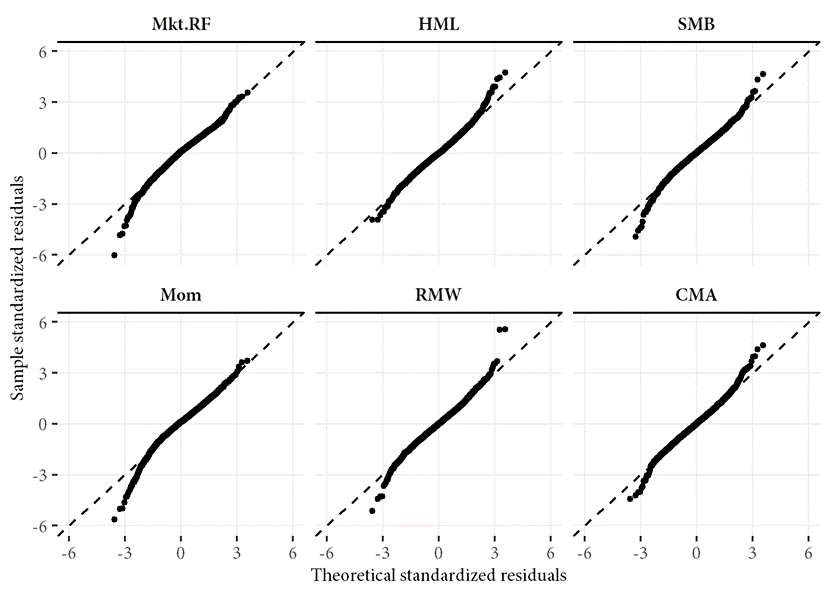
\includegraphics[scale = 1]{graphics/qq_norm.png}
  \centerline{(i) Normal innovations} \\
  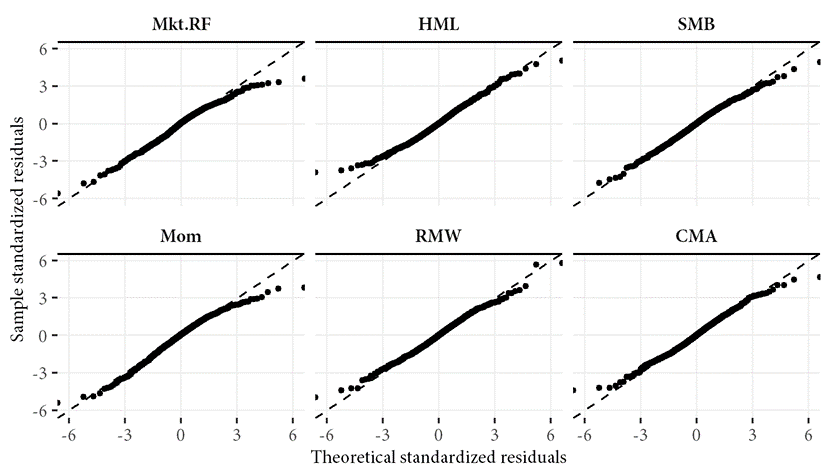
\includegraphics[scale = 1]{graphics/qq_std.png}
  \centerline{(ii) Student's \textit{t} innovations} \\
  %\bottomrule
  \vspace{3mm}
  \footnotesize
  Quantile-quantile plots of theoretical standardized residuals and standardized residuals from the best (lowest BIC) ARMA-GARCH model specifications. Data from the theoretical distribution should line up on the dashed line. Based on weekly data 1963-2016
  \end{minipage}
\end{figure}

\begin{figure}[htbp]
  \caption{QQ-plots on residuals from ARMA-GARCH with skewed Student's \textit{t} innovations}
  \label{fig:qq_ghst}
  %\toprule
  \centering
  \begin{minipage}{\textwidth}
  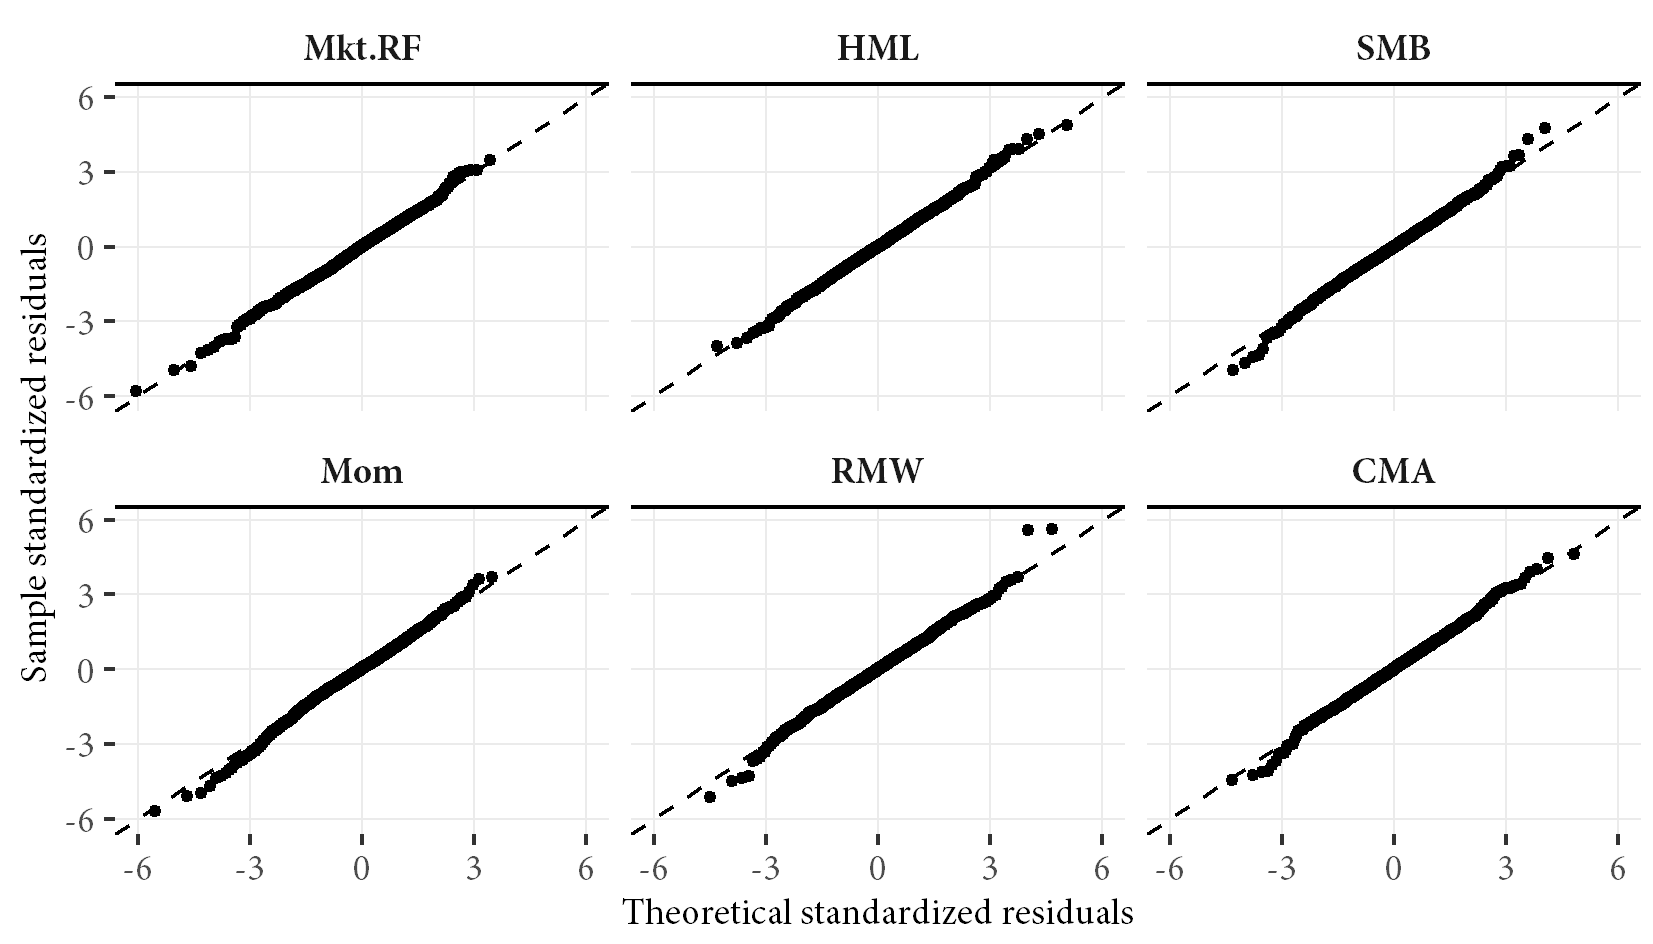
\includegraphics[scale=1]{graphics/qq_ghst.png}  
  %\bottomrule
  \vspace{3mm}      
  \footnotesize
  Quantile-quantile plots of theoretical (skewed Student's \textit{t}) standardized residuals and standardized residuals from the best (lowest BIC) ARMA-GARCH model specifications. Data from the theoretical distribution should line up on the dashed line. Based on weekly data 1963-2016
  \end{minipage}
\end{figure}

In the variance equation, all factors exhibit high $\alpha$ and $\beta$ leading to a high variance persistence, between 0.96 and 0.99. Generally, variance persistence, which is related to volatility clustering, tends to be high in financial return series. [WHAT DOES IT MEAN WHY DO I CARE] We note that the zero-cost factor portfolios are no exception. The HML factor has a higher $\alpha$ estimate, indicating that shocks of equal size translate into slightly stronger volatility for HML than for RMW and CMA. RMW, on the other hand, has both the lowest $\alpha$ estimate and the highest $\beta$ estimate, indicating higher persistence and lower sensitivity of volatility to shocks.

We note that the Mkt-RF factor is, according to our model selection procedure, best fitted by a ARMA(0, 0) mean equation, indicating no predictive power of 1-week lagged returns. Also, in the variance equation, we note that the relatively low $\alpha = 0.037$ sensitivity to shocks is increased considerably by $\eta = 0.181$ in the case of a \emph{negative} shock. Furthermore, the Mom factor stands out with a much higher estimate of $\alpha$ (0.186) than any of the other series (all around 0.10) and a lower $\beta$ (0.793). This means that volatility in the momentum factor is more sensitive than other factor strategies to return shocks and less predictable by past volatility alone. We also note that the Mkt-RF and Mom factors exhibit relatively higher unconditional volatilities (of 0.022 and 0.018) than do other factors (around 0.010).

For both the value-related and non-value related factors, many of the estimates of $\gamma$, the skewness of the skewed Student's \textit{t} GARCH innovation process, are statistically insignificant. This is also the case for the degree of freedom estimates for SMB and Mom. Although these parameters are not significantly estimated, we believe that including them is essential as QQ-plots (\autoref{fig:qq_norm_std}) indicate misspecification for models with both the normal and Student's \textit{t} innovations.

% section modeling_factor_returns (end)
